\section{Results}
\label{sec:results}

\subsection{Did the roles fire?}
\label{sec:did-fire}

In Figure~\ref{fig:checks} we perform the check for each role against the length-matched neutral
condition on 200 development items, in a paired bootstrap with 2,000 resamples (and no missing data,
across all 3,600 invocations). \textbf{Only one in six roles accomplishes its stated operation:}
counter-evidence checking more than doubles the rate of counterclaims and flagging relative to a
length-matched neutral instruction ($d = 1.03$). This check is a sum of two components and they do
not move together: explicit counterevidence items rise ($d = +1.48$ here, $+0.95$ on the second
family) while flagged claims fall, significantly so on the second family ($d = -0.33$).
Appendix~\ref{app:robustness} decomposes every check that has two parts.

\textbf{Two registered statistics are negative.} The explore-then-prune condition results in
\emph{less} hypothesis diversity compared to one with no explicit instructions ($d = -0.95$). The
local-claim checker finds \emph{fewer} claims compared to no explicit instructions ($d = -0.18$),
but its guard is effectively constant (1,191 of 1,200 records; invariant in every operation arm), so
we report but do not interpret this statistic as a validated reversal. As shown in Panel~(b), the
companion factor is saturated in both product rules. Thus explore-then-prune reflects a genuine
reversal rather than a within-metric tradeoff, while local-claim effectively collapses to a
one-factor check; Appendix~\ref{app:concedes} records this limitation.

\textbf{Three roles are statistically indistinguishable from neutral} ($|d| < 0.07$, $p > 0.36$).
\emph{Note: the null distribution for the rare hypothesis check does not reflect the full strength
of its safeguard against hallucinated hypotheses, which is based on the difference between unsourced
and sourced statements. Because sourcing approaches saturation in these records, this safeguard has
no effect, and the null is not as strong a baseline as for a check where the safeguard was
effective.}

\begin{figure}[t]
\centering
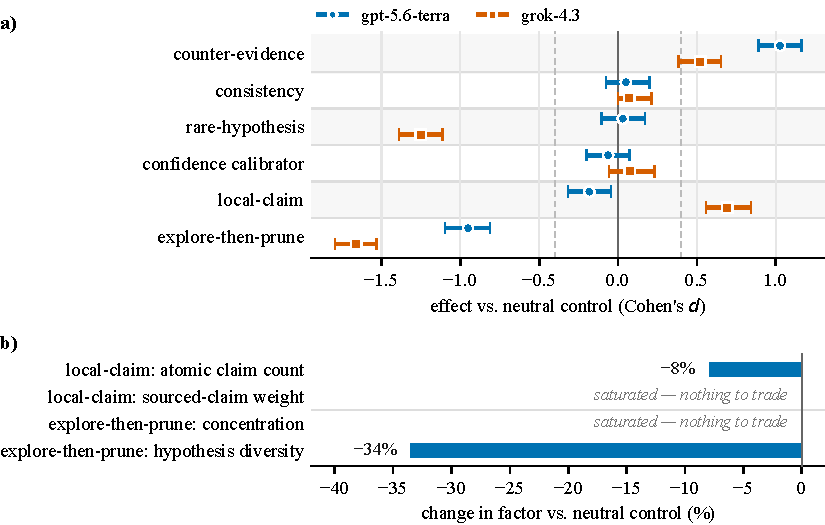
\includegraphics[width=\linewidth]{figures/checks_panel.pdf}
\caption{(a) Standardized difference of stated role effect against length-matched neutral condition,
on 200 datapoints, in two pretraining families, with 95\% bootstrap confidence intervals. Dashed
lines at pre-registered $|d| \ge 0.40$. (b) These flips are not tradeoffs because both measures are
product rules, with the factor being traded against pinned to maximum in both arms of the
experiment, leaving all the action to the factor we told it to increase.}
\label{fig:checks}
\end{figure}

\begin{table}[t]
\centering
\small
\begin{tabular}{llll}
\toprule
Check & Degeneracy named & Audit & Status \\
\midrule
counter-evidence      & ---                      & no guard was specified            & unguarded \\
consistency           & flag all, then abstain   & flag all and \emph{answer} scores 1.0 & defeatable \\
confidence calibrator & lower confidence blindly & constant shifts lower ECE         & defeatable \\
local-claim           & emit unchecked claims    & constant in 1,191/1,200 records   & collapsed \\
explore-then-prune    & breadth without resolution & concentration $\approx 1$ throughout & inactive \\
rare-hypothesis       & fabricate alternatives   & penalty $\approx 0$ throughout     & unexercised \\
\bottomrule
\end{tabular}
\caption{Each check's guard against the strategy it was written to exclude. Three failure classes
appear: guards that never vary, guards a cheap strategy defeats, and a check with none.}
\label{tab:guards}
\end{table}

\subsection{Auditing the guards}
\label{sec:audit}

A check is only as informative as the guard meant to stop a degenerate strategy passing it. We
stress-tested each against the strategy it names (Table~\ref{tab:guards});
Appendix~\ref{app:concedes} works the defeatable cases through.

\textbf{These audits were not pre-registered and do not replace the pre-registered check statistics;
they constrain their interpretation.} The statistics in \S\ref{sec:did-fire} stand; what the audit
withdraws is the licence to read them as construct-valid measurements --- including the one that
passes, which has no guard against fabricated counterevidence.

\subsection{The pattern replicates across families}
\label{sec:replication}

We designed these checks under a major assumption not yet verified: that the findings generalize
across models, and reflect something about the role prompting approach. To test this, we replicated
all six checks on the same 200 development examples for another pretraining family
(\texttt{grok-4.3}). The results are plotted in Figure~\ref{fig:checks}(a).

\textbf{The overall finding replicates.} The general finding that most role prompts do not score
well on their own check (one out of six, and two out of six) \emph{is} a property of the role
prompting approach at this scale, not just of a single model. Setting aside the local-claim check,
whose guard is constant in 1,191 of 1,200 records and which we therefore do not treat as a validated
instrument (Appendix~\ref{app:concedes}), the count is one of five on both families. The flip
replicates and becomes more pronounced: in both pretraining families, the \emph{explore-then-prune}
approach yields lower hypothesis diversity than a prompt specifying no particular approach, now with
a $d = -1.66$ on the second model as well. The single exception replicates as well: in both cases,
the only effective role was that of checking for counter-evidence.

\begin{table}[t]
\centering
\small
\begin{tabular}{lp{0.44\linewidth}l}
\toprule
 & does not move the benchmark & moves the benchmark \\
\midrule
passes its check & counter-evidence checking & --- \\
fails its check  & consistency checking, local-claim checking, explore-then-prune,
                   rare-hypothesis checking, confidence calibration & --- \\
\bottomrule
\end{tabular}
\caption{Registered two-axis classification across all six roles. The right-hand column is empty
because no role clears the pre-registered 0.05 leave-one-out threshold. Due to that, no role moved a
benchmark score \emph{without} passing its operational check --- a statement the check makes
available and a benchmark delta alone cannot. The local-claim row is retained for pre-registration
transparency; \S\ref{sec:audit} withdraws its instrument-level interpretation.}
\label{tab:twoaxis}
\end{table}

\textbf{Which roles fire does \emph{not} replicate.} Two of six change sign. Local claim checking
fails for one of these, and succeeds for the other. Rare hypothesis checking has no effect for one
of these and is highly reversed for the other. These are large effects. None of this difference is
due to one group being noisier than the other; three of these differences survive correction
($q = 0.016, 0.00075, 0.00075$). The one exception is the rare-hypothesis checking on
\texttt{gpt-5.6-terra} ($q = 0.71$), the null reported above. On the five checks we treat as
validated, this is one of five rather than two of six: local-claim checking is the other sign
change, and its reversal is a property of a check that reduces to a bare claim count, so the
non-transfer rests on rare-hypothesis checking alone. That remains a large non-transfer (null on one
family and $d = -1.25$ on the other) but it is one role, not two.

This is the strongest available argument for the tool. Had every role failed everywhere, the finding
would reduce to a list of prompts to avoid. Because at least one validated role-specific check
differs substantially across the two families tested, role behaviour should be validated on the
target model rather than assumed to transfer. We report two families and claim nothing about a
third.

The pre-registered binary classification --- does the role pass check, does it affect the benchmark
(Table~\ref{tab:twoaxis}) --- ends up in a single cell. The interpretation of this cell depends on
the asymmetry reported in A2.5. If a role affects the score \emph{despite} failing the check, this
is direct evidence for the claims of this paper --- an effect on the benchmark which is decoupled
from the claimed function. If a role \emph{passes} the check and has no effect, then this is a less
clear signal, as it is muddled with the detection issue (our detectable effect size at
$n = 1{,}000$ is 0.048, with SESOI 0.03; there could still be an effect which is just below the
floor).

Our pre-registration specifies that differences between arms should be reported as absolute effects,
rather than relative to some unknown gain (see Appendix~\ref{app:cross-arm}). These are informative
nulls, rather than inconclusive studies: with intervals of half-width $\approx 0.01$, we can be
confident that the full operational instructions prompt provides less than $\approx 1$ accuracy
point relative to either the operation names prompt or no operation, and the two operation prompts
have a zero difference. Similarly, the trained synthesiser also finds no extra value (see
Appendix~\ref{app:synth}).

\textbf{The only statistically detectable behavioural difference across arms is refusal, and it does
not affect these contrasts.} We never see refusal from an agent role on any HaluEval question in any
arm, so the comparisons are all across a constant, full set of questions. Refusal occurs only on
TruthfulQA, where the persona names prompt rejects significantly less than both controls: the mere
presence of a name can affect rejection rates with no distinct operation to attribute it to --- the
confounding mechanism we raise concern about in this paper, observed only on unscored questions
(Appendix~\ref{app:refusal}).

\textbf{There is no difference between council and single call.} Councils always perform \emph{worse}
than a single direct model query on all 1,000 scored questions, by $-0.015$ to $-0.022$ points, with
corrected intervals excluding zero. The effect sizes are smaller than H1's pre-registered 0.03
SESOI, so we claim councils do not outperform a single call, not that they are meaningfully worse;
and our baseline is a same-model single-call baseline rather than cost-matched (\S\ref{sec:arms}).
Appendix~\ref{app:single-call} gives both tie rules.

\textbf{Agents give high-confidence predictions whether they are correct or not.} Average reported
confidence is 0.982 against actual accuracy of 0.848, yet confidence is meaningfully associated with
correctness (AUROC 0.716) --- real signal squashed into the highest percentiles. Reported confidence
carries information about answer correctness but does not validate execution of the requested
operation (\S\ref{sec:did-fire}). The squashing is lineage-specific. \textbf{Exploratory}, not
pre-registered (Appendix~\ref{app:confidence}).

We perform the pre-registered attribution study via leave-one-out retraining of all candidates (full
council vs.\ six different drop-one coalitions, seven trainings total, see
Appendix~\ref{app:loo} for details). \textbf{No role makes a difference.} The maximum leave-one-out
difference in magnitude is 0.016, well below the pre-registered threshold of 0.05 (less than a third
as large), and all ranges include zero. These results are essentially null (5 different values for
different coalitions, so not a degeneracy) but also directionally biased toward zero (leave-one-out
penalizes every interaction with the council with that role, skewing differences down, making them
conservative) and none are near the threshold such that the conservative bias would be relevant.

\textbf{For one of the two pre-registered tests, we have no data.} The FDR family testing agent-role
pairs against their primary benchmark assigns one role (the one role whose primary benchmark
survived scoping) to TruthfulQA --- upon which it scores zero. Half of this FDR family's cells are
missing, meaning the corrected $q$-values are indeterminate and we do not report them (rather than
just returning the HaluEval column).

We do not (and do not report null findings for) the primary council-improvement hypothesis or H2.
The scoped analysis is, by design, underpowered to detect the primary hypothesis. Similarly, for
five of six roles, their pre-registered primary target is removed by the dual-benchmark reduction;
the LOO results are thus per-role results on HaluEval, which is no role's pre-registered primary
target. Finding one for H2 would be precisely the kind of result-switching we oppose in this work.
For the manipulation checks only, the results generalise across families. Only one family has data
for the two benchmarks, LOO analysis, or single-call comparison.
